\documentclass{article}

\usepackage{graphicx}
\usepackage{tikz}
\usepackage{tikzsymbols}
\usetikzlibrary{calc,patterns,shapes.geometric}
\pagestyle{empty}
\usepackage[margin=0pt]{geometry}
\geometry{papersize={14in,12in}}

\def\centerarc[#1](#2)(#3:#4:#5){\draw[#1] ($(#2)+({#5*cos(#3)},{#5*sin(#3)})$) arc (#3:#4:#5);}

\begin{document}
	\begin{figure}
		\centering
		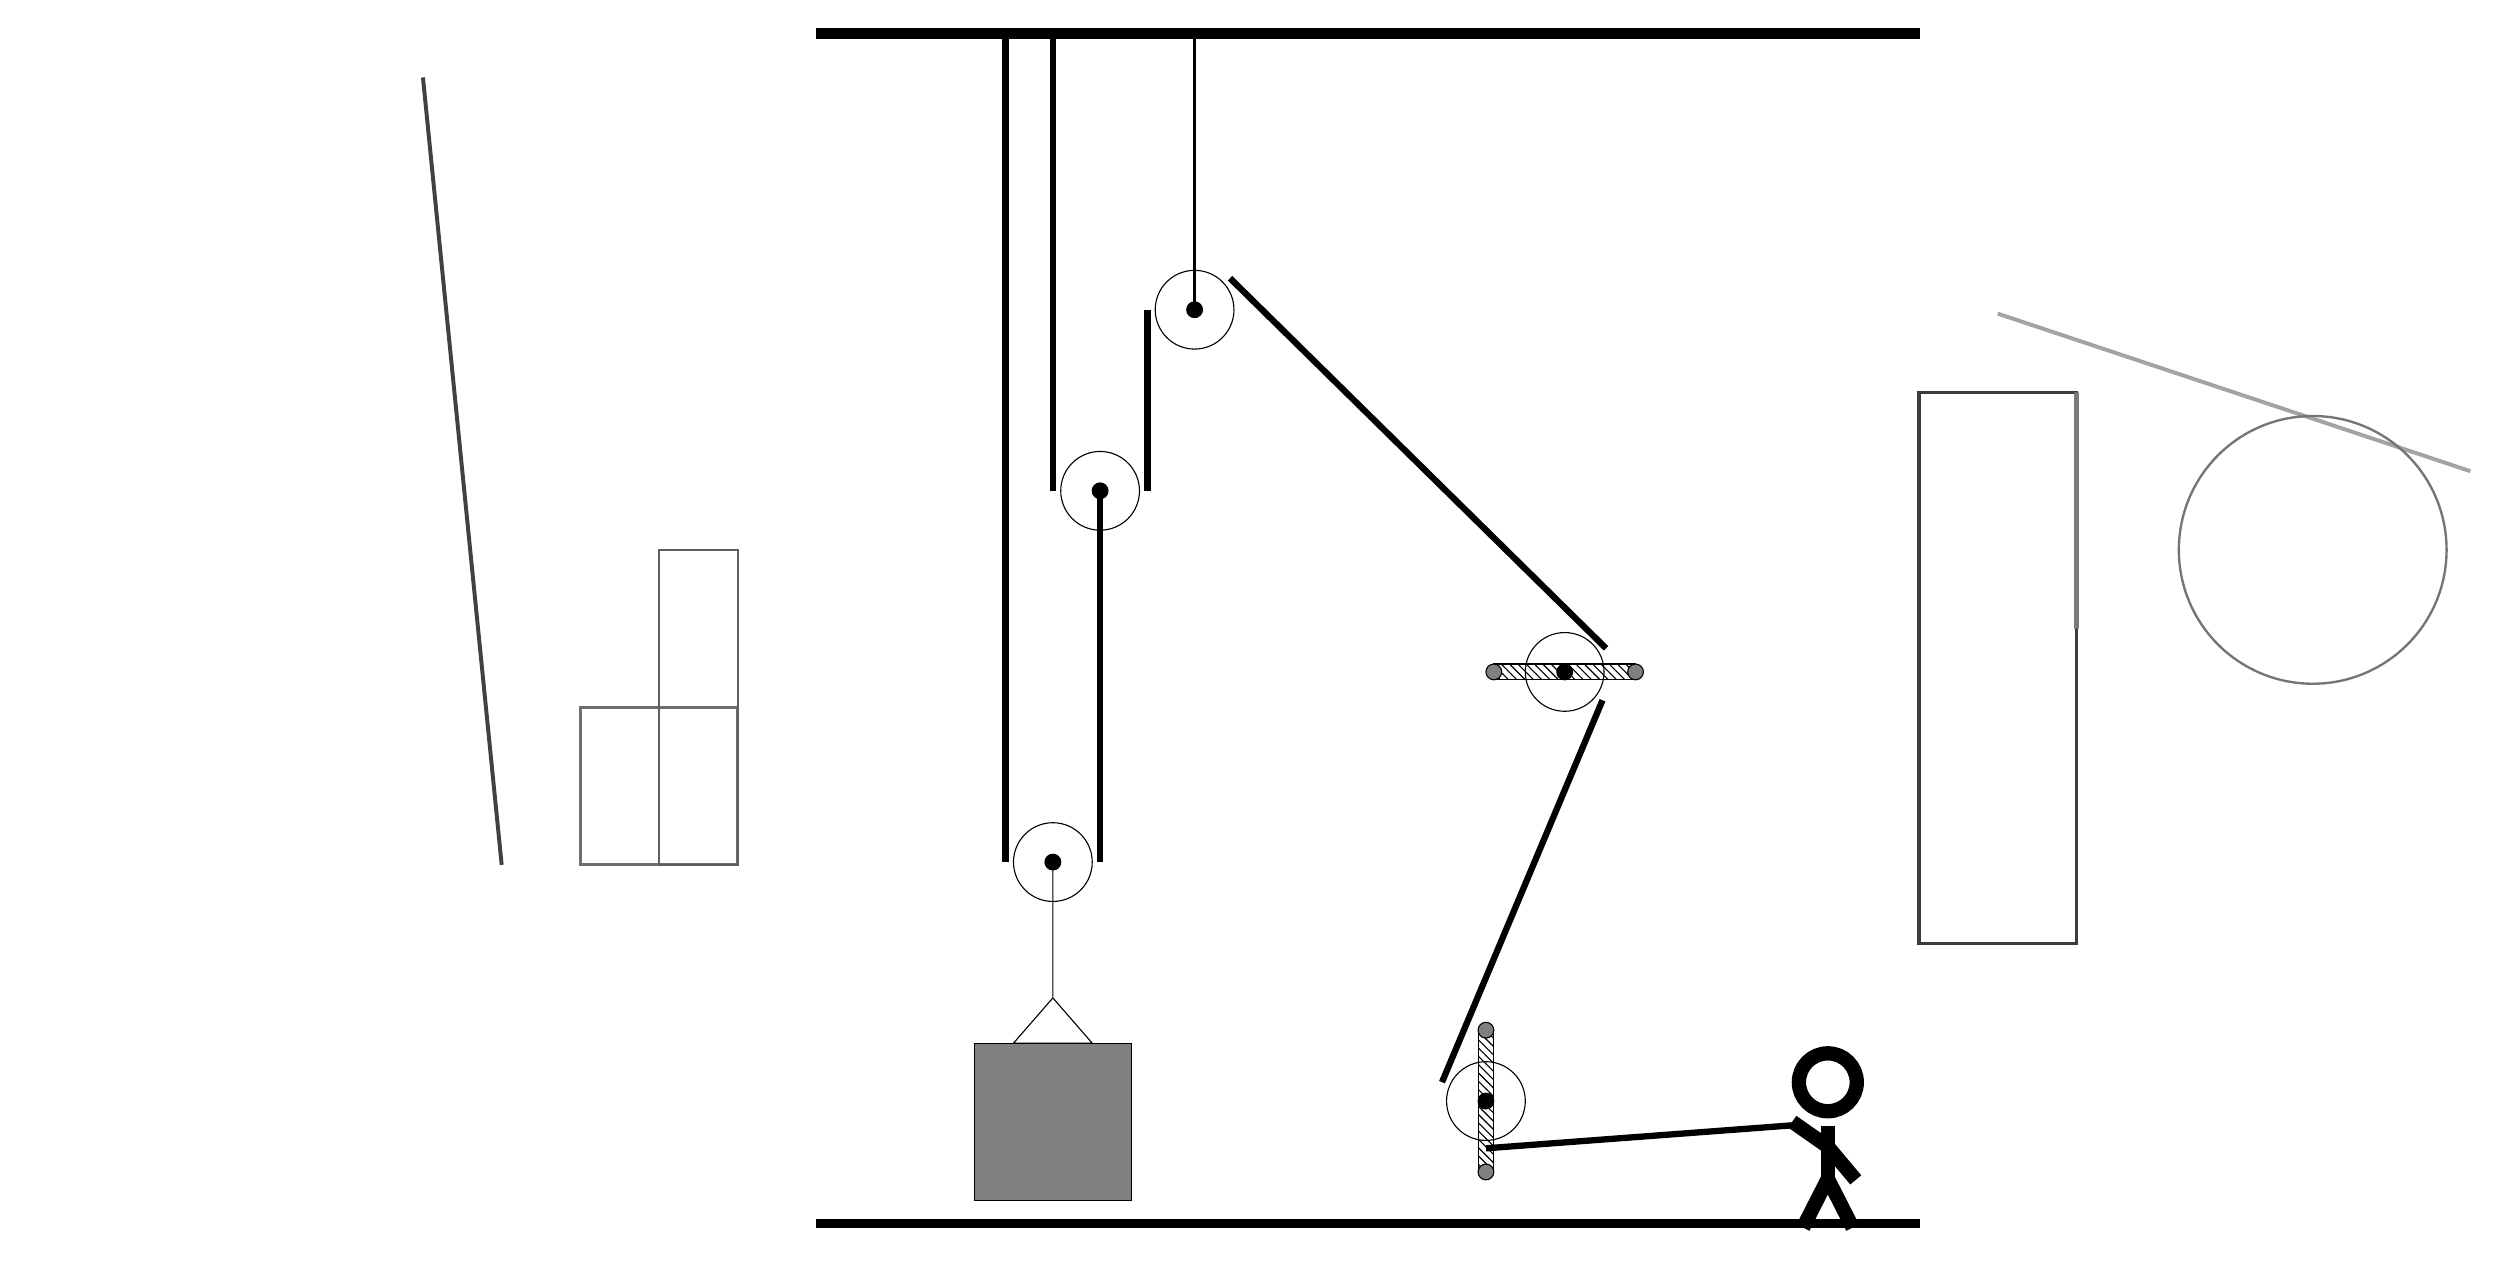
\begin{tikzpicture}
			%%%%% START %%%%%
			
			\draw[fill=black] (-2, 11.5) rectangle (12, 11.625);
			
			\draw (1, 1.035) circle (0.5);
			\draw[fill=black] (1, 1.035) circle (0.1);
			
			\draw (1.6, 5.75) circle (0.5);
			\draw[fill=black] (1.6, 5.75) circle (0.1);
			
			\draw (2.8, 8.05) circle (0.5);
			\draw[fill=black] (2.8, 8.05) circle (0.1);
			\draw[thick] (2.8, 8.05) -- (2.8, 11.5);
			
			\draw (6.5, -2) circle (0.5);
			\draw[fill=black] (6.5, -2) circle (0.1);
			\draw[pattern=north west lines, pattern color=black] (6.4, -1.1) rectangle (6.6, -2.9);
			\draw[fill=black!50] (6.5, -1.1) circle (0.1);
			\draw[fill=black!50] (6.5, -2.9) circle (0.1);
			
			\draw (7.5, 3.45) circle (0.5);
			\draw[fill=black] (7.5, 3.45) circle (0.1);
			\draw[pattern=north west lines, pattern color=black] (6.6, 3.55) rectangle (8.4, 3.35);
			\draw[fill=black!50] (6.6, 3.45) circle (0.1);
			\draw[fill=black!50] (8.4, 3.45) circle (0.1);
			
			\draw (1, 1.035) -- (1, -0.69) -- (0.5, -1.265) -- (1.5, -1.265) -- (1, -0.69);
			\draw[fill=black!50] (0, -1.265) rectangle (2, -3.265);
			
			\draw[line width=0.8mm] (0.4, 11.5) -- (0.4, 1.035);
			\centerarc[line width=0.8mm](1, 1.035)(180:360:0.6);
			\draw[line width=0.8mm](1.6, 1.035) -- (1.6, 5.75);
			\draw[line width=0.8mm] (1.0, 11.5) -- (1.0, 5.75);
			\centerarc[line width=0.8mm](1.6, 5.75)(180:360:0.6);
			\draw[line width=0.8mm](2.2, 5.75) -- (2.2, 8.05);
			\centerarc[line width=0.8mm](2.8, 8.05)(35:180:0.6);
			\draw[line width=0.8mm] (3.25, 8.45) -- (8.025, 3.75);
			\centerarc[line width=0.8mm](7.5, 3.45)(215:135:-0.6);
			\draw[line width=0.8mm](7.98, 3.09) -- (5.942, -1.76);
			\centerarc[line width=0.8mm](6.5, -2)(-30:100:-0.6);
			\draw[line width=0.8mm](6.5, -2.6) -- (10.5, -2.3);
			
			\node at (10.8, -2.5) {\Strichmaxerl[10][-35][-50]};
			
			\draw[line width=0.5mm, color=black!36](13, 8) -- (19, 6);
			
			\draw [line width=0.3mm, color=black!54](17, 5) circle (1.7);
			\draw[line width=0.5mm, color=black!75](-7, 11) -- (-6, 1);
			\draw[line width=0.4mm, color=black!57] (-3, 1) rectangle (-5, 3);
			\draw [line width=0.4mm, color=black!32](-12, 11) circle (0.0);
			
			\draw[line width=0.4mm, color=black!77] (12, 0) rectangle (14, 7);
			
			\draw[line width=0.7mm, color=black!52] (14, 7) rectangle (14, 4);
			\draw[line width=0.3mm, color=black!63] (-3, 5) rectangle (-4, 1);
			
			\draw[fill=black] (-2, -3.5) rectangle (12, -3.6);
			
			%%%%% END %%%%%
		\end{tikzpicture}
	\end{figure}	
\end{document}